\documentclass[10pt,a4paper]{article}

\usepackage{graphicx}
\usepackage[left=2.5cm,right=2.5cm,top=2.5cm,bottom=2.5cm]{geometry}
\usepackage{geometry}
\usepackage{pdflscape}
\usepackage{amsmath}
\usepackage{amsfonts}
\usepackage{amssymb}

\begin{document}
\title{Work Plan for the Selection of the $\mu$Reactor Design at UIUC\\}
\author{Draft\\ \\ \\ \\ Kathryn D. Huff,\\
Mehmet Turkmen,\\
Zoe Richter}
\date{\today}
\maketitle

\pagebreak
\section{Introduction}
Micro-reactors are the reactors which produce power typically less than 20 MWe and site less than 500 m2 (0.1 acre) in the size of shipping container or a big house. They are considered to be automated operation with minimum operating staff. Due to the small size and low consequences of micro-reactors, the regulations applied to the existing (non)commercial reactors may not fully applicable to micro-reactors. Apart from other advanced reactor designs like SMRs, micro-reactors have specific following licencing issues: security, aircraft strike, emergency preparedness, source term analysis, staffing, remote operation, decommissioning, transportation, manufacturing licenses, quality assurance, probabilistic risk assessment and NRC oversight.

\section{Reactors} \label{sec:reactors}
Nine designs of micro-reactors are under investigation: Westinghouse (eVinci), Holosgen (Holos), LANL (MegaPower), MicroNuclear, NuScale (NuScale), Oklo (Oklo), Starcore (Starcore), Urenco (U-battery) and X-energy (Xe-100) (in alphabetical order). Kairos does not have any reactor designs which produce power less than 200 MWe. A brief comparison of the selected reactors is listed in Table \ref{microreactors}. In addition, recent progresses in the design reviews of different reactors around the world are provided in Table \ref{reviews}. 

The information on reactor designs was mainly gathered from the following sources.

1. International and domestic government organization databases: design information was collected from the International Atomic Energy Agency (IAEA), the Nuclear Energy Agency (OECD-NEA), the U.S Department of Energy (U.S. DOE), and the U.S.
Nuclear Regulatory Commission (U.S.NRC) online databases.

2. Vendor database: the latest design brochures, catalogues and reports were directly obtained from the vendors.

Notes:

1. GA is developing a mobile nuclear power supply that is truck/air shippable and would fit in a standard military shipping container. This modular, autonomous system has a load-following generating capacity of up to 10 MWe and a refueling period greater than 10 years. (source: press releases)

2. The NuGen Engine developed by NuGen is a direct-cycle gas-cooled microreactor. The concept design, by Professor Tsvetkov at the Department of Nuclear Engineering at Texas A$\&$M University, produces 1-50 MWe scalable output. It is in the stage of patent aproaval. (source: https://www.nucdev.com/about-us.html)

3. In the case of MSR design at micro-level, only Terrapower has started to adopt its MCFR design to 1-10 MWe with more than 10 years refueling.(source: press releases of the president) 

\pagebreak
\newgeometry{margin=1cm}
\begin{landscape}
\begin{table} [ht]
\begin{center}

\caption{A brief comparison of micro-reactor designs}
\label{microreactors}
\begin{tabular}{|l|l|l|l|l|l|l|l|l|}
\hline 
Design 		&eVinci 		& Holos		&MegaPower 	& NuScale		& Oklo 		& Starcore		& U-battery 		& Xe-100 \\ 
\hline 
Institution 	&Westinghouse& Holosgen	&LANL	& NuScale		& Oklo Inc. 	& Starcore		& Urenco 		& X-energy \\ 
Source 	&\cite{Levinsky18};\cite{Yan20};\cite{Arafat19}  &\cite{holos17}  	& \cite{mega15};\cite{mega17}	& \cite{NuChapter4} 		& \cite{Oklofsar} 	&\cite{starwebsite} 		&\cite{Ubattery}  		&\cite{IAEA18};\cite{xmeeting} \\ 
Type			&Heat Pipe	& HTGR (Pebble)	  	& Heat Pipe 		& PWR/Heat Pipe&Heat Pipe   			&	HTGR (Pebble)			& HTGR (Pebble)	& HTGR (Pebble)\\ 
Spectrum		&Epithermal	& Thermal 		 	&Fast  	&Thermal/Thermal 		&Fast   			& Thermal  			&	Thermal		&Thermal\\ 
Power (MWe)	&0.2-5		& 10/13  			&2			& 10-50 /1-10			& $\backsim$2  			&2x10  			&4-8			&75\\ 
Refueling (years)&5 to 10		&12 or 20   			&	5		& 2/- 			& 12 (estimated)  			&5  			&5-10 			&Online refueling\\ 
Enrichment (\%)&19.75		&8 for 12 or 15 for 20   			&19.75			& $<$4.95/- 		&  5 to 20 			&$<$20	  			&20-17			&15.5\\ 
Core  Diameter (m)	&1.5		& 1.8  			&1.5			& 1.5/- 		&   			&1.5   			&3.5-1.8			& 5\\ 
Fuel			&UN/U-Mo	& UCO TRISO  			&	UO2		&UO2/-		&  U-Zr 			& UCO TRISO  			&UCO TRISO			&UCO TRISO\\ 
Clad			&-		&  Silicon carbide 			&	-		& M5/- 		&   -			&Silicon carbide   			&Silicon carbide			&Silicon carbide\\ 
Heat Pipe fluid	&Na/K	& -  			&K			& - 		& Na/K 			&  - 			&	-		&-\\ 
\hline
\end{tabular}

\caption{Worldwide design reviews}
\label{reviews}
\begin{tabular}{|l|l|l|l|l|l|}
\hline 
	 &Country of Origin 	& Company		&Reactor type			&Output(MWe) 	& Status \\ 
\hline 
1 	&Canada/US		& Terrestrial Energy	&Molten Salt Integral	&200		& PHASE 1 COMPLETED \\ 
 	&		& 	&	&		& PHASE 2 PENDING  \\
2 	&US/Korea/China	& UltraSafe Nuclear	&High-temperature gas prismatic block	&5		& PHASE 1 IN PROGRESS completion date 2018   \\ 
 	&		& /Global First Power	&	&		& PHASE 2 Service Agreement under development  \\
3 	&Sweden/Canada	&LeadCold	&Molten lead pool fast spectrum	&3-10		& PHASE 1 ON HOLD AT VENDOR REQUEST  \\ 
4 	&US		&Advanced Reactor Concepts	&Sodium pool fast spectrum	&100		& PHASE 1 IN PROGRESS  \\ 
5 	&UK		&U-Battery	&High temperature gas prismatic block	&4		& PHASE 1 Service Agreement under development  \\ 
6 	&UK		&Moltex Energy	&Molten salt fast spectrum	&300		& PHASE 1 IN PROGRESS  \\ 
7 	&Canada/US		&StarCore Nuclear	&High-temperature gas prismatic block	&10		& PHASE 1 and 2 Service Agreement under development   \\ 
8 	&US		&SMR, LLC. &Pressurized Water	&160		&PHASE 1 Service Agreement under development   \\ 
 	&		& (A Holtec International Company)		&	&		&  \\
9 	&US		&NuScale Power	&Integral Pressurized Water	&50		&PHASE 2* Service Agreement under development   \\ 
10 	&US		&Westinghouse Electric Co.	&eVinci Micro Reactor	&$<$25		&PHASE 2* Service Agreement under development  \\ 
11 	&Japan		&4S	&Na cooled fast reactor	&10		&Licensing pre-application  \\ 
12 	&Russia		&ABV	&PWR	&2x7.9		&Part of design licensed  \\ 
13 	&Argentina	&CAREM-25	&PWR	&27		&Licensing in progress  \\ 
14 	&Russia		&KLT-40S	&PWR	&2x35	&Licensed and under construction  \\ 
\hline
\end{tabular}

\end{center}
\end{table}
\end{landscape}
\restoregeometry

\pagebreak
\subsection{Westinghouse}
Full design details have not been revealed yet for public; only general information is given by the company. However, several academic studies, most of them eVinci-like, can be found in the literature. Recently, two papers, \cite{Xu19} and \cite{Wright19}, have been published in 18th NURETH conference. Those are not available for now but reaching them somehow would be valuable. Westinghouse is planning to finalize the current design of eVinci by 2022, testing by 2023 and commercializing by 2025. Hernandez et al. \cite{Hernandez19} performed a series of calculations in eVinci-like (not eVinci) for natural resource utilization, burnup analyses, waste management and environmental impacts. The details of eVinci design obtained from the documents published by Westinghouse are presented in Table 3. Reactor core configuration and 3D design representation are given in Figs. \ref{eVincidesign} and \ref{eVincioverview}.

\begin{table} [ht]
\begin{center}

\caption{eVinci design parameters}
\begin{tabular}{l  l  l}
\hline
Design 		&Value (from Westinghouse reports) 		& Value (other) \cite{Hernandez19}\\ 
	& 	\cite{IAEA18};\cite{Levinsky18};\cite{Yan20};\cite{Arafat19} 	&  \\ 
\hline
Core Diameter (in) 		&59.06 		&  \\ 
Monolith materials 		& 		& Type-316 SS	\\ 
Refueling (years) 		&Up to 10 		&  \\ 
Fuel 		&UN/U-Mo 		& 	 \\ 
Fuel Pellet Density, \% TD 		&96 		&  \\ 
Enrichment (\%) 		&19.75 		&  \\ 
Fuel channel radius (in) 		& 		& 0.281 \\ 
Number of fuel channels 		&378 (1 MWth), 4219 (14 MWth)		& 2112 (5 MWth) \\ 
Reflector material 		&		& BeO\\ 
HP channel radius (in) 		&		& 0.298\\ 
Number of HP channels 		& 		& 1224\\ 
HP to HP web thickness (in) 		& 		& 0.039\\ 
Fuel to fuel web thickness (in) 		& 		& 0.059\\ 
HP total length (ft) 		&		& 13.12\\ 
HP fluid 		&Na/K		& \\ 
HP fluid temperature (K) 		&920 		& \\ 
\hline

\end{tabular}
\end{center}
\end{table}

\begin{figure}[hbtp]
\centering
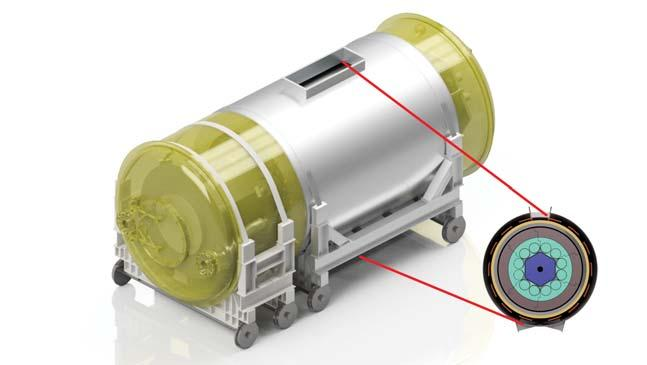
\includegraphics[scale=0.5]{Figs/evincicore.jpeg}
\caption{eVinci Core Configuration}
\label{eVincidesign}
\end{figure}

\begin{figure}[hbtp]
\centering
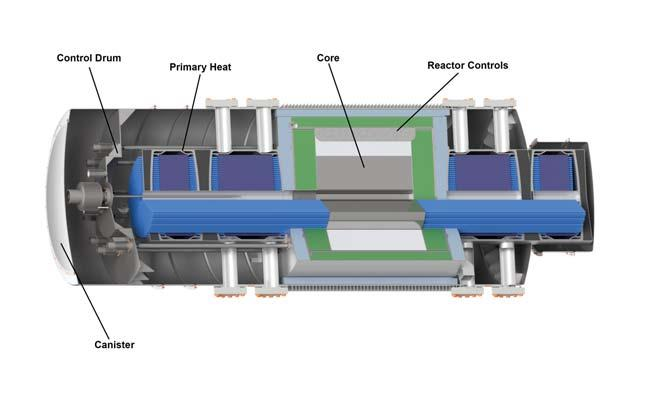
\includegraphics[scale=0.5]{Figs/evinciover.jpeg}
\caption{eVinci Micro Reactor Overview}
\label{eVincioverview}
\end{figure}

\pagebreak
\subsection{Holosgen}
Holos design uses four subcritical fuel cartridges as given in Fig. \ref{Holosquad}. TRISO fuels fill the fuel channels, as illustrated in Fig. \ref{Holosdesign}. Complete design details including radiation protection and shielding, and safety are available in \cite{holos17}.

\begin{table} [htbp]
\begin{center}

\caption{Holos core geometry and composition}
\label{Holostable}
\begin{tabular}{l     l}
\hline 
Design 		&Value \\ 
\hline 
Reactor thermal power (MWt)&22                                             \\
U-235 enrichment (wt\% )&8-15             \\
Whole core volume (m3)&6.9                                        \\
\hline 
Fuel Channels&19x4                      \\
Fuel Channel Diameter (cm)&1.4            \\
Coolant Channels&54x4                   \\
Coolant Channel Diameter (cm)&0.7               \\
Brick Graphite Density (g/cm3)&2.23              \\
Brick Edge Length (cm)&6               \\
Brick Height (cm)&10             \\
\hline 
UO2 Density  (g/cm3) & 10.8                       \\
Kernel Diameter  (cm) & 0.05                       \\
Buffer Layer Thickness  (cm) & 0.01            \\
SiC, IPyC, OPyC Thickness  (cm) & 0.012   \\
TRISO Sphere Diameter  (cm) & 0.094         \\
Total core bricks & 1,925                           \\
Packing Fraction (\%) & 70                       \\
\hline 
TRISO spheres in one fuel channel  &24,778   \\
TRISO spheres in one brick            &470,777 \\
TRISO spheres in core  &3.62x10$^{9}$            \\
\hline 
Temperature Coefficient of Reactivity -$\rho_{T}$- (pcm)&-8       \\
Delayed Neutron Fraction -$\beta_{eff}$- (pcm)&733      \\
Generation Time -$\Lambda$- ($\mu$s)&233                        \\
\hline 

\end{tabular}
\end{center}
\end{table}

\begin{figure}[hbtp]
\centering
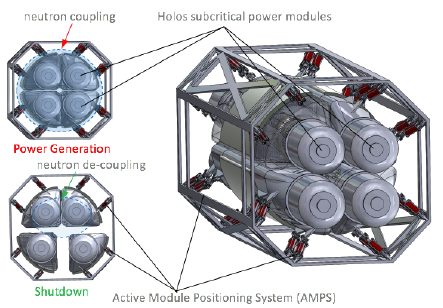
\includegraphics[scale=1]{Figs/holosquad.jpeg}
\caption{Holos Quad generator}
\label{Holosquad}
\end{figure}

\begin{figure}[hbtp]
\centering
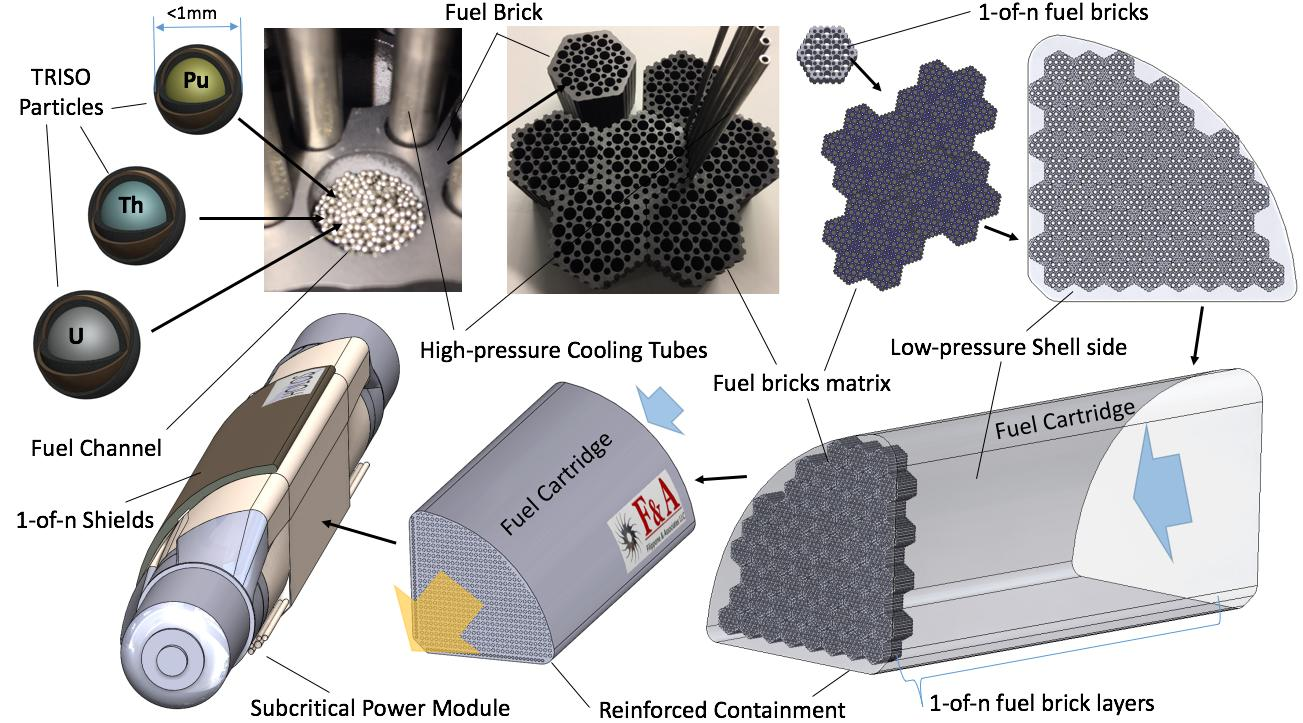
\includegraphics[scale=0.3]{Figs/holosfueldesign.jpeg}
\caption{Holos subcritical assembly design}
\label{Holosdesign}
\end{figure}

\pagebreak
\subsection{LANL}
MegaPower is a Los Alamos National Laboratory (LANL) reactor design concept. Table \ref{Megatable} provides important features of MegaPower reactor parameters. More specific design details can be found in the reports \cite{mega17} and \cite{mega15}. Results of the neutronics and thermal-hydraulics analyses have been published by INL and LANL in various reports. Apart from 5 MWt design, there is an advanced 15 MWt design which uses UN fuel and Na as HP fluid. However, publications are mostly on the first design shown in Figs. \ref{Megadesign} and \ref{Megaoverview}. 

\begin{figure}[hbtp]
\centering
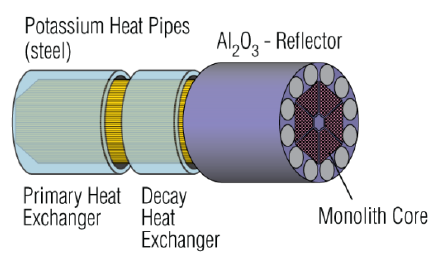
\includegraphics[scale=0.8]{Figs/megacore.jpeg}
\caption{Megapower concept design}
\label{Megadesign}
\end{figure}

\begin{figure}[hbtp]
\centering
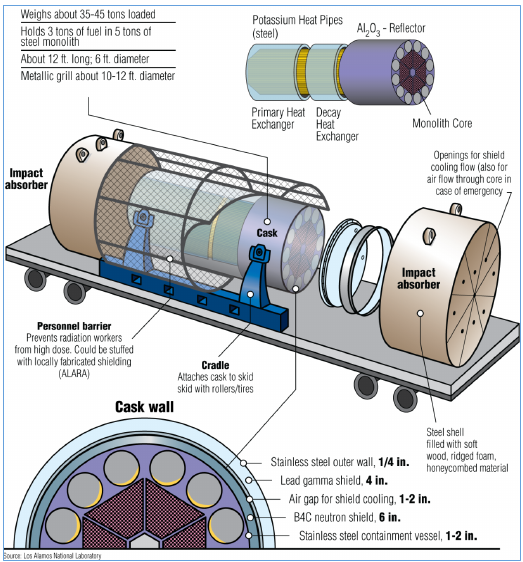
\includegraphics[scale=0.7]{Figs/megacask.jpeg}
\caption{Megapower reactor overview}
\label{Megaoverview}
\end{figure}

\pagebreak
\begin{table} [hbtp]
\begin{center}

\caption{MegaPower Reactor Core Description}
\label{Megatable}
\begin{tabular}{l     l}
\hline 
Design 		&Value \\ 
\hline 
Reactor thermal power&5 MW                                             \\
Reactor electrical power output&2 MW(e)                                       \\
Reactor core orientation&Horizontal                                       \\
Cycle length&5 years                                           \\
Coolant system&Heat pipes                                      \\
Reactor structure&Type 316 Stainless steel monolith    \\
\hline 
Fuel Form&UO2                      \\
Theoretical density&10.96 g/cm3           \\
Percent of theoretical density&96.0\%                   \\
U-235 enrichment&19.75 wt\%             \\
Fuel channel hole outer diameter&1.425 cm               \\
Fuel pellet geometry&Cylindrical              \\
Fuel pellet outer diameter&1.412 cm               \\
Gas gap thickness&0.0065 cm             \\
Fuel rod length&150.0 cm               \\
Fuel-to-fuel pitch&1.60 cm                 \\
Fuel-to-HP pitch&1.60 cm                 \\
Gas&Helium                   \\
Gas pressure&20 atmospheres   \\
Number of fuel rods in-core&2,112                     \\
\hline 
Number of HPs in-core&1,224         \\
HP hole diameter (in-core)&1.575 cm    \\
HP-to-HP pitch&2.7713 cm  \\
HP working fluid&Potassium  \\
HP total length&4.0 m         \\
HP isothermal temperature&675°C        \\
\hline 
Monolith material&Stainless steel (SS316)       \\
Monolith steel density&8.03 g/cm3                         \\
Monolith edge thickness (HP-to-edge)&2 mm                                 \\
Web thickness between HP-to-fuel holes&0.100 cm                            \\
Web thickness between fuel-to-fuel holes&0.175 cm                            \\
Web thickness between HP-to-edge of block&0.150 cm                            \\
\hline 
Side reflector material&Alumina (Al2O3)       \\
Alumina density&3.9 g/cm3                        \\
Side reflector outer radius&77.85 cm                                 \\
Side reflector radial thickness&21-29 cm                            \\
Top/bottom reflector material&SS316 + BeO                            \\
\hline 
Number of control drums&12       \\
Number of emergency control rods&2       \\
Control material&B4C                        \\
\hline 

\end{tabular}
\end{center}
\end{table}

\pagebreak
\subsection{MicroNuclear}
There is absolutely nothing on MsNB design of MicroNuclear LLC company. I think this company has a weak desire to go into the micro-nuclear world. 


\subsection{NuScale}
Detailed technical specifications (as seen in Table \ref{Nutable}) related to reactor core design, source term, licensing requirements and safety assessments are given in the NRC web-page \cite{NuChapter19}. This is the FSAR for the SMR design of NuScale. NuScale considers two different micro-reactor concepts \cite{nichol19}: one (10-50 MWe) is based on current small modular reactor tecnhnology and the other (1-10 MWe) is based on heat pipe reactor technology. The first one is very similar to the SMR. FSAR report  seems quite sufficient by supplying all the details about the plant. 2D and 3D views of the reactor are illustrated in Figs. \ref{Nu2d} and \ref{Nu3d}, respectively. This design can be altered for the $\mu$R concept of NuScale for a nominal electric power of less than 20 MW. There is no detail on the heat pipe design.  \\
In 2018, BWX Technologies was selected to provide manufacturing input. In 2019, Doosan Heavy Industries and Construction and NuScale signed an MOU. 

\begin{table} [htbp]
\begin{center}

\caption{NuScale Reactor Core Description \cite{NuChapter4}}
\label{Nutable}
\begin{tabular}{l     l}
\hline 
Design 		&Value \\ 
\hline 
Core diameter (in)			&59.25\\
Active fuel height (in)	&78.74\\

Number of FA 		&  37\\
Rod array   			&17x17\\
Fuel assembly length (in) &  94\\
Fuel assembly pitch (in)	&8.466\\
Fuel rod pitch (in)&0.496\\
Number of spacer grids&5\\
Grid height (in)&1.75\\
Number of Fuel rods&264\\
Number of Guide tubes&24\\
Number of Instrumentation tubes&1\\
\hline 
Number of FR&264\\
Diametral gap (in)&0.0065\\
Cladding material&M5\\
Cladding outside diameter (in)&0.374\\
Cladding inside diameter (in)&0.326\\
Cladding thickness (in)&0.024\\
Fill gas&helium\\
\hline 
Fuel Pellet Density, \% TD&96\\
Material&UO2 (sintered)\\
Diameter (in)&0.3195\\
Length (in) &0.40\\
\hline 
Number of CR Assemblies&16                              \\
Upper absorber material&boron carbide              \\
Lower absorber material&silver-indium-cadmium \\
Cladding&304 stainless steel      \\
Fill gas&helium                        \\
\hline 
BA Material Type&integral with fuel         \\
Material &gadolinia (Gd2O3 )      \\
Number &Up to 32 per assembly\\
\hline 
Nuclear Design Parameters (for Equilibrium Cycle)\\
Core Average Linear Power (kw/ft)&2.5     \\
Total Heat Flux Hot Channel Factor&1.860  \\
Nuclear Enthalpy Hot Channel Factor&1.386  \\
\hline 
Reactivity Coefficients\\
Doppler temperature coefficient (pcm/F)&-1.4 to -2.25\\
Moderator temperature coefficient (HZP-HFP) (pcm/F)&+6 to -43     \\
Boron coefficient (pcm/ppm)&-10             \\
\hline 
Effective Delayed Neutron Fraction 
and Prompt Neutron Lifetime\\
$\beta_{eff}$ BOC&0.0059\\
$ \beta _{eff}$ EOC&0.0052\\
Prompt lifetime BOC (10-6 seconds)&18.35  \\
Prompt lifetime EOC (10-6 seconds)&-6       \\
\hline 
Boron Concentration (BOC) (ppm)&2000\\
\hline 

\end{tabular}
\end{center}
\end{table}

\begin{figure}[htbp]
\centering
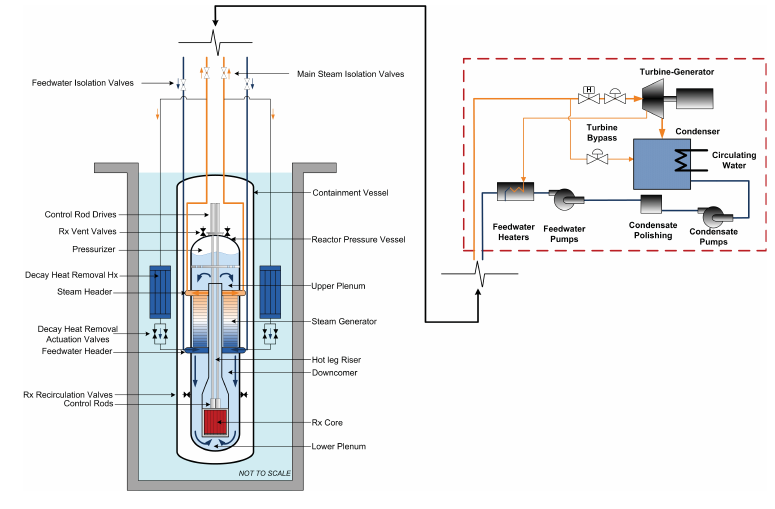
\includegraphics[scale=0.7]{Figs/nuscale2d.jpeg}
\caption{ Two-dimensional schematic of a single NuScale unit}
\label{Nu2d}
\end{figure}

\begin{figure}[htbp]
\centering
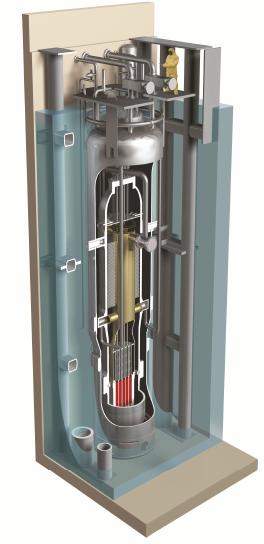
\includegraphics[scale=0.8]{Figs/nuscale3d.jpeg}
\caption{NuScale 3D SMR view}
\label{Nu3d}
\end{figure}

\pagebreak
\subsection{Oklo}
Oklo is working on a Compact Fast Reactor design since 2013. Since November 2016, NRC has been engaged in pre-application activities (the docket number - 99902046) with Oklo. Public version of the final safety analysis report of Oklo \cite{Oklofsar} is not enough for the understanding of the reactor design. Full version has the details such as probabilistic risk assessment, release pathway and enviromental impact but was closed to public access. Even company web site is unreachable. The company is now making collaboration with ANL and INL. 

\subsection{Starcore}
The StarCore technical data is acquired directly from the vendor website and summarized in Table \ref{startable} below. In terms of size and basic technical characteristics, the reactor, illustrated in Fig \ref{Starcore}, is similar to HTR-10, a prototype pebble bed modular reactor built and operated in China, and HTTR, a 30 MWth experimental gas cooled reactor in Japan.

HTGR reactor with 2 reactor units per standard plant is embedded 15m underground in Ultra High Strength Concrete (UHSC) silos. The reactors are installed in silos 57 metres deep (as seen in Fig. \ref{Starview}) and 13 metres in diameter, made from double-walled high performance concrete with a steel canister silo at the base.  TRISO fuel compacts supplied by BWX Technologies. StarCore is fully automated and has only two operating states: Load Following and Shutdown.

\begin{figure}[htbp]
\centering
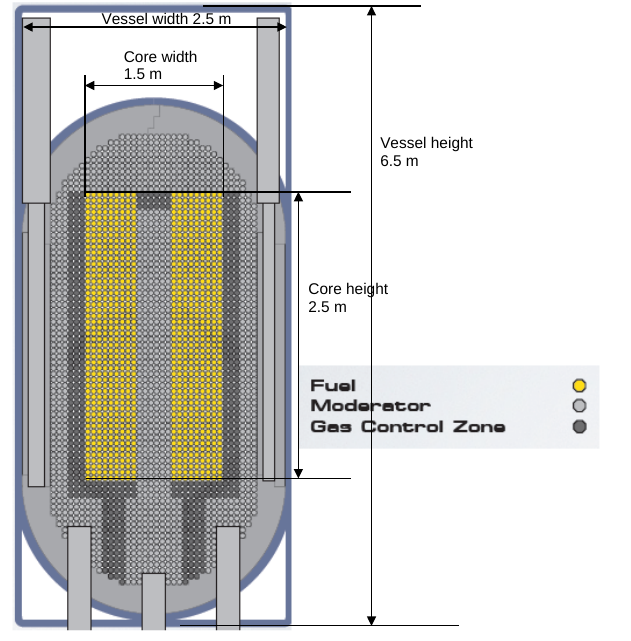
\includegraphics[scale=0.5]{Figs/starcorereactor.jpeg}
\caption{StarCore reactor core}
\label{Starcore}
\end{figure}

\begin{figure}[htbp]
\centering
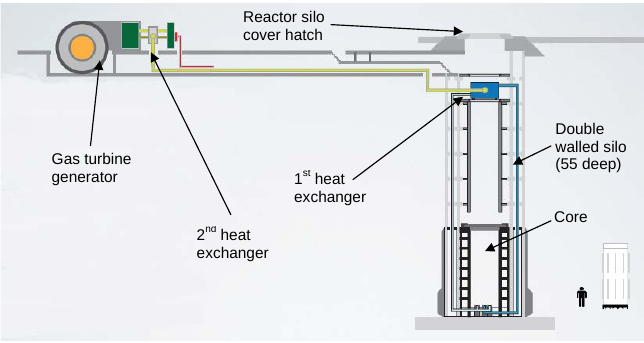
\includegraphics[scale=0.7]{Figs/starcoreview.jpeg}
\caption{Side view of Starcore}
\label{Starview}
\end{figure}

\begin{table} [ht]
\begin{center}

\caption{ StarCore reactor design}
\label{startable}
\begin{tabular}{l l}
\hline 
Design 		&Value \\ 
\hline 
Core Diameter (m) 		&1.5 \\ 
Core Height (m) 		&2.5 \\ 
Refueling (y)		&  5 (off-site)\\ 
Fuel		&UCO TRISO Pebbles \\ 
Enrichment (\%)		&$<$20 \\ 
Number of fuel pebbles		&26,800 \\ 
Number of TRISO particles per pebble		&2,000 \\ 
Pebble fuel core diameter (mm)		&60 \\ 
Fuel element geometry & Truncated cuboctahedron\\ 
Cladding material & Silicon carbide \\ 
Primary side coolant 	&Helium \\ 
Core outlet temp (C) 	&850 \\ 
Core operating pressure (MPa)	&7.5 \\ 
Secondary side coolant	&Nitrogen \\ 
Secondary side operating pressure (MPa)	&6.8 \\ 
\hline 

\end{tabular}
\end{center}
\end{table}

\pagebreak
\subsection{Urenco}
The concept design, namely U-battery, has been made by the Universities of Manchester, Dalton Institute (UK) and Technology University of Delft (Netherlands). There is strong desire to operate the reactor by 2026. Main design parameters \cite{Ubattery} are tabulated in Table \ref{Utable}. A 3D view and core layout of the reactor are displayed in Figs. \ref{u3d} and \ref{ucore}. 

\begin{table} [htbp]
\begin{center}

\caption{U-battery design}
\label{Utable}
\begin{tabular}{l l l}
\hline 
Design 		&10 MWe &20 MWe\\ 
\hline 
Reflector composition & BeO          &  Graphite\\
Control rods (\#) & 4                        &  6 \\
Fuel Blocks (\#) & 6*4                     & 30*4 \\
Enrichment (\%) & 20                      & 17  \\
Fuel life time (a)&  5                       & 10  \\
Fuel block dimension (cm) & 36*80 &  36*80 \\
Fuel mass (kg) & 208                     &   1.040\\
Burn-up (MWd/kg HM)  & 88           &   70 \\
\hline 
Outer diameter (cm)             &   180  &  370   \\
Vessel thickness (mm)        &   $<$100       & 100   \\
Reactor core diameter (cm)  &   108     &  252  \\
Reflector thickness (cm)      &   20 (BeO)    &29    \\
Insulation thickness (cm)     &   5 (SiC fiber)     & 10 (SiC fiber)   \\
Barrel thickness (cm)           &    2   & 2    \\
Gap thickness (cm)             &    5  &  5  \\
\hline 
Core Height (cm)          & 320         & 320 \\
Top reflector (cm)         &  20 (BeO)&50  \\
Bottom reflector (cm)    &  20 (BeO)& 50 \\
Top plenum (cm)          &20            &20  \\
Bottom plenum (cm)     &  50          &50  \\
Top insulation (cm)       &30           &30 \\
Bottom insulation (cm)  &  60         &60 \\
Core support plate (cm) &  10         &15  \\
Support structure (cm)  &   60         &60  \\
Vessel height (cm)       & 590         &655  \\
\hline 
BeO mass (kg) &    7.900       &0  \\
Graphite mass (kg) &   8.100        & 70.000  \\
Flask inner diam (cm)& 180       & - \\
Flask inner height (cm)& $<$500         & - \\
\hline 

\end{tabular}
\end{center}
\end{table}


\begin{figure}[htbp]
\centering
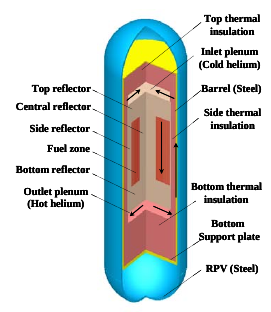
\includegraphics[scale=1]{Figs/ubattery3d.jpeg}
\caption{ 3D reactor configuration of U-battery}
\label{u3d}
\end{figure}

\begin{figure}[htbp]
\centering
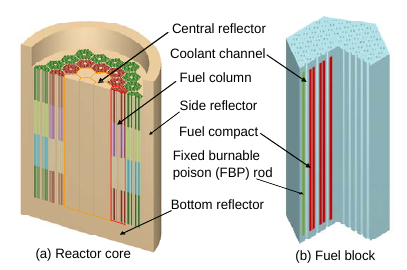
\includegraphics[scale=1]{Figs/ubatterycore.jpeg}
\caption{ Core and fuel block of U-battery}
\label{ucore}
\end{figure}

\pagebreak
\subsection{X-energy}
X-energy company provides various reactor designs ranging from 600 MWt to 30 MWt, called as Pebble Bed Fuel Reactor. The main micro-rector design is ST-OTTO (refering to Fig.  \ref{xo}) which produces 30-48 MWt power. But the design details are not open for public. I think the design is very identical to the design of 200 MWt, as presented in Table \ref{xtable} except for the reactor size and fuel type. Th-based fuel is under consideration for the use in TRISOs. 

\begin{table} [ht]
\begin{center}

\caption{ X-energy design}
\label{xtable}
\begin{tabular}{l l}
\hline 
Design 		&Value \\ 
\hline 
Core Diameter (m) 		&4.88 \\ 
Core Height (m) 		&20 \\ 
Refueling		&Online fuel loading  \\ 
	&175 fresh pebbles/day \\ 
Fuel		&UCO TRISO Pebbles \\ 
Enrichment (\%)		&15.5 \\ 
Number of fuel pebbles		&220,000 \\ 
Number of TRISO particles per pebble		&18,000 \\ 
Pebble fuel core diameter (mm)		&50 \\ 
Pebble diameter (mm)	&60 \\ 
Number of passes		&60\\ 
Final burnup (GWd/tHM)		&160 \\ 
Burnable poison		&no \\ 
Power density (MW/m3)		&4.8 \\ 
UCO TRISO kernel diameter (mm)	&0.425 \\ 
Porous Carbon Buffer thickness (mm)	&0.095 \\ 
Inner Pyrolytic Carbon Layer thickness (mm) 	&0.04 \\ 
Silicon Carbide Layer thickness (mm)	&0.035 \\ 
Outer Pyrolytic Carbon Layer thickness (mm)	&0.04 \\ 
Core Inlet temp (C)	&259 \\ 
Core Outlet temp (C) 	&750 \\ 
Core Inlet Pressure (MPa)	&6 \\ 
Core Outlet Pressure (MPa)	&5.84 \\ 
\hline 

\end{tabular}
\end{center}
\end{table}

\begin{figure}[hbtp]
\centering
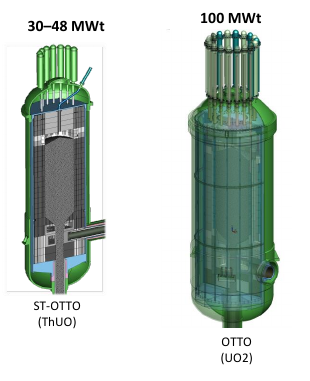
\includegraphics[scale=0.97]{Figs/xoverview.jpeg}
\caption{X-energy micro-reactor overview}
\label{xo}
\end{figure} 

\pagebreak
\section{Site Requirements}
For site requirement, main documents are: 

1. Idaho National Laboratory, “Modernization of Technical Requirements for Licensing of Advanced Non-Light Water Reactors, Probabilistic Risk Assessment Approach,” Rev 0, August 2019.

2. Idaho National Laboratory, “Modernization of Technical Requirements for Licensing of Advanced Non-Light Water Reactors, Selection and Evaluation of Licensing Basis Events,” Rev 0, August 2019.

3. Idaho National Laboratory, “Modernization of Technical Requirements for Licensing of Advanced Non-Light Water Reactors, Safety Classification and Performance Criteria for Structures, Systems and Components,” Rev 0, August 2019.

4. Idaho National Laboratory, “Modernization of Technical Requirements for Licensing of Advanced Non-Light Water Reactors, Risk-Informed and Performance-Based Evaluation of Defense-inDepth Adequacy,” Rev 0, August 2019.

\pagebreak
\section{Source Term}
A general source term analysis comprises transient scenario modeling, fuel pin radionuclide distribution, failed pin radionuclide release, radionuclide bubble transport, offsite dispersion analysis and containment region analysis. Some of them can, however, be eliminated or new ones can be added depending on which micro-reactor is to be chosen. As an example, the micro-reactor design does not include any spent fuel storage, thus the source term would not.
For the source term analysis of a selected micro-reactor design, phenomena and release paths of accident scenarios first need to be identified. Pathways for some advanced reactors (i.e., HTGR, SFR, MSR) are illustrated in Fig. \ref{pathway}. There are on-going discussions in the NRC on the evaluation of the source term of micro-reactors; it is expected to come to a conclusion on the licencing issues including the source term by the end of this year (estimated). 

\begin{figure}[hbtp]
\centering
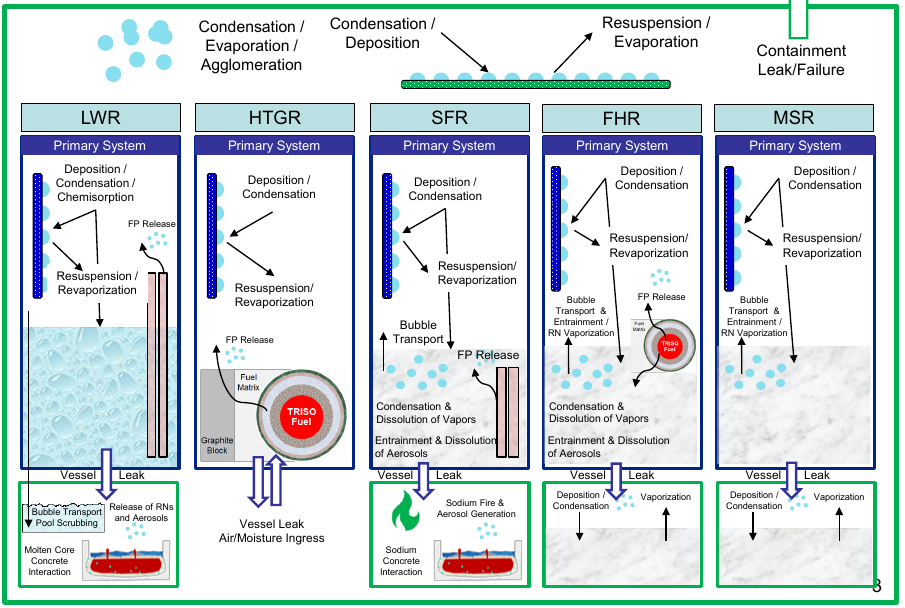
\includegraphics[scale=0.6]{Figs/pathway.jpeg}
\caption{Pathway for radioactive release for several reactor types}
\label{pathway}
\end{figure}

There is a possibility to make an assumption for the pathway identification of the micro-reactors. We can use the same or modified pathways of the existing reactors, accepted by the NRC, for the analogy to the selected micro-reactor design. Yet, heat pipe reactors may still require as the release ways have not completely known.
The method for the source term calculation recommended by the NRC is given in Fig. \ref{sourceterm}. The method to be applied changes with the type of the reactor. In any cases, MELCOR, system accident analysis code, produce the source term for the defined design-basis accidents. 
For probabilistic offsite consequence analysis bounded by the calculated source term, MACCS code needs to be utilized. The code is capable of evaluating the Level 3 PRA including the radionuclide release, atmospheric transport, meteorology, protective actions, site data, dosimetry, health effects, economic factors, and so forth. Design-specific and site-related issues must be input to the code.  Meteorological statistics (i.e., day and night temperatures, magnitude and direction of the wind, tornados, flooding level), topographical data and population density and distribution, habitat of the animals and the location of the endemic plants are to be recorded.   
The methodology and the results on the source term calculations are presented in detail in the relevant documents of NuScale \cite{NuChapter19} and eVinci \cite{Southern19}.

\begin{figure}[hbtp]
\centering
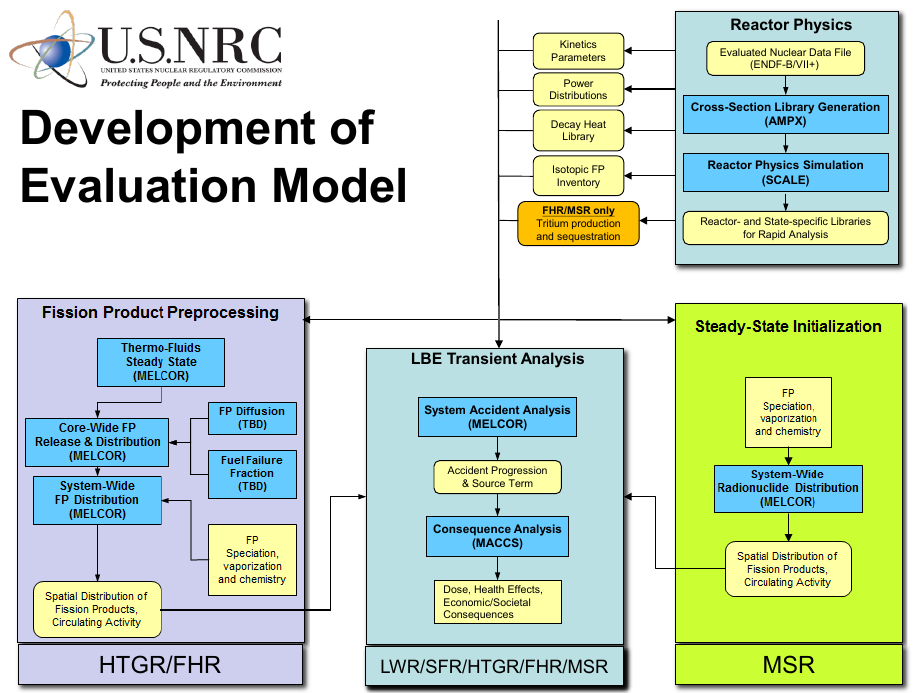
\includegraphics[scale=0.6]{Figs/sourceterm.jpeg}
\caption{Source term evaluation model}
\label{sourceterm}
\end{figure}

According to the NuScale, the potential radionuclide source term associated with a severe accident is much smaller (5\%) than that associated with a 1000 MWe design. This value is 1\% for eVinci. 

\pagebreak
\section{Licencing Procedure}
For the licensing of the research reactors, below documents are critical:

1. Guidelines for Preparing and Reviewing Applications for the Licensing of Non-Power Reactors: Standard Review Plan and Acceptance Criteria (NUREG 1537, Part 2).

2. Guidelines for Preparing and Reviewing Applications for the Licensing of Non-Power Reactors: Format and Content (NUREG 1537, Part 1). 


https://www.nrc.gov/reading-rm/doc-collections/nuregs/staff/sr1537

A reference document \cite{nichol18} has discussed  the micro-reactor from the various acpects inculding waste management, fuel supply and action plans.


\section{Safety Assessment}
This part is going to be discussed later but will include accident scenarios including design-basis that a nuclear facility must be designed and built to withstand, and beyond design accidents that are possible but were not fully considered in the design process.

\section{Discussion on the Report}

Considering available data of the interested reactors given in Section \ref{sec:reactors}, full core modeling capabilities are presented in Table \ref{table:feasiblity}. it should be taken into account that desing details of the reactor to be selected can be gathered from the corresponding vendor. What should be the criteria for the selection of the micro-reactor?

1. according to reactor type
2. according to NRC review
3. 

\begin{table} [ht]
\begin{center}

\caption{Full core modeling}
\label{table:feasiblity}
\begin{tabular}{|l|l|l|l|l|l|l|l|l|}
\hline 
Design 		&eVinci 		& Holos		&MegaPower 	& NuScale		& Oklo 		& Starcore		& U-battery 		& Xe-100 \\ 
\hline 
$\times$ or 	$\surd$ 		&  $\times$		& $\surd$		& $\surd$ 	&   $\surd$		&  $\times$		& $\surd$	&  $\surd$ 		&  $\surd$ \\ 
\hline 

\end{tabular}
\end{center}
\end{table}

\pagebreak
\section{Conclusion}

\pagebreak
\begin{thebibliography}{X}
\bibitem{Xu19} Hong, X., Jurie J.,  van W., Richard F., W., 2019. Thermal Analysis for eVinci Micro™ Reactor. Presented at the 18th International Topical Meeting on Nuclear Reactor Thermal Hydraulics (NURETH18), Portland, OR.
\bibitem{Wright19} Wright, R.F., Dokmanovich, A.M., 2019. Phenomena Identification and Ranking Table for the eVinciTM Micro Reactor. Presented at the 18th International Topical Meeting on Nuclear Reactor Thermal Hydraulics (NURETH18), Portland, OR.
\bibitem{Yan20} Yan, B.H., Wang, C., Li, L.G., 2020. The technology of micro heat pipe cooled reactor: A review. Annals of Nuclear Energy 135, 106948. https://doi.org/10.1016/j.anucene.2019.106948
\bibitem{Arafat19} Yasir Arafat, Jurie Van Wyk, “Nuclear Plant Journal: eVinci™ Micro Reactor – Our Next Disruptive Technology,” http://www.westinghousenuclear.com/Portals/0/new%20plants/evincitm/eVinci%20Micro%20Reactor%20NPJ%20M-A%202019.pdf?ver=2019-04-30-211410-367
\bibitem{Hernandez19} Hernandez, R., Todosow, M., Brown, N.R., 2019. Micro heat pipe nuclear reactor concepts: Analysis of fuel cycle performance and environmental impacts. Annals of Nuclear Energy 126, 419–426. https://doi.org/10.1016/j.anucene.2018.11.050
\bibitem{NuChapter4} NuScale, “NuScale Standard Plant Design Certification Application - Chapter 4: Reactor, Part 2-Tier 2”, Revision 2, ML18310A325, October 2018. https://www.nrc.gov/reactors/new-reactors/design-cert/nuscale.html. 
\bibitem{Southern19} Southern Company, “Modernization of Technical Requirements for Licensing of Advanced Non-Light Water Reactors: Westinghouse eVinciTM Micro-Reactor Licensing Modernization Project Demonstration”, DOE, SC-29980-202, 2019.
\bibitem{NuChapter19} NuScale, “NuScale Standard Plant Design Certification Application: Chapter Nineteen Probabilistic Risk Assessment and Severe Accident Evaluation”, Rev. 2, 2018. 
\bibitem{Levinsky18} Levinsky, A., Wyk, J.J., Arafat, Y., et al., 2018. Westinghouse eVinci Reactor for Off-Grid Markets. Transactions of the American Nuclear Society, Orlando, Florida, November 11-15.
\bibitem{IAEA18} IAEA, “Advances in Small Modular Reactor Technology Developments A Supplement to: IAEA Advanced Reactors Information System (ARIS)”, 2018. 
\bibitem{Ubattery}Ding, M., Kloosterman, J.L., Kooijman, T., Linssen, R., 2011. Design of a U-Battery (No. PNR-131-2011-014). Urenco, and Koopman and Witteveen.
\bibitem{starwebsite} http://starcorenuclear.ca
\bibitem{xmeeting} Harlan, B., 2018. X-energy Xe-100 Reactor initial NRC meeting, AccessionNumber=ML18253A109. 
 https://adamswebsearch2.nrc.gov/webSearch2/main.jsp?.
\bibitem{mega17}  Sterbentz, J.W., Werner, J.E., Hummel, A.J., Kennedy, J.C., Wright, R.N., Biersdorf, J.M., 2017. Special Purpose Nuclear Reactor (5 MW) for Reliable Power at Remote Sites Assessment Report: Using Phenomena Identification and Ranking Tables (PIRTs) (No. INL/EXT-16-40741). Idaho National Laboratory Nuclear Science and Technology Division.
\bibitem{mega15}  McClure, P., Poston, D., Rao, D.V., Reid, R., 2015. Design og MegaWatt Power Level Heat Pipe Reactors (No. LA-UR-15-28840). Los Alamos National Laboratory.
\bibitem{holos17}  Filippone, C., Jordan, K.A., 2017. The Holos Reactor: A Distributable Power Generator with Transportable Subcritical Power Modules. 
\bibitem{nichol18} Nichol, M., 2018. Roadmap for the Deployment of Micro-Reactors for U.S. Department of Defense Domestic Installations (Technical Report). Nuclear Energy Institute.
\bibitem{nichol19} Nichol, M., 2019. Cost Competitiveness of Micro-Reactors for Remote Markets (Technical Report). Nuclear Energy Institute.
\bibitem{Oklofsar} Oklo, Inc., 2018. Pilot Application for DG-1353, Enclosure 1 (Submittal to Support NRC Development and Implementation of DG-1353, A Guidance to Risk-Inform Application Development and Contents Including Event Selection and SSC Classification No. Oklo-2018-R10-NP, Rev 0), Pilot Application. Oklo, Inc.



\end{thebibliography}

\end{document}
